\section{MLP}
In this section, we will introduce the first model, which we will refer to as the
baseline model, based on a Multi-Layer Perceptron.
We will analyze its architecture, the training phase, and its final performance.

%In questa sezione andremo ad introdurre il primo modello a cui faremo
%riferiento come baseline model, basato su MultiLayer Perceptron.
%Analizzeremo la sua architettura, la 
%fase di training e le sue performance finali.

\subsection{Architecture}
This neural network is designed to predict the instantaneous energy output over
a period of exactly 2 days.
To do this, it requires input data that includes the performance of the system
(features selected during the Preprocessing phase, see Chapter \ref{chap:datapreprocessing}) for exactly one day
before and one day after the period in question.
This enables it to understand how the system is performing and,
consequently, provide the energy output trend.
The model consists of 6 main layers:

%Questa rete neurale è progettata per prevedere l'andamento dell'energia istantanea prodotta durante un periodo di un buco di esattamente 2 giorni.
%Per farlo ha bisogno di avere come input l'andamento dell'impianto (features selezionate nella fase di preprocessing) di esattamente un giorno prima del
%buco e di un giorno dopo. In questo modo può riuscire a comprendere come l'impianto sta performando e quindi restituire l'andamento dell'energia.
%Il modello è formato da 6 livelli principali:

\begin{figure}[H]
	\begin{minipage}{0.6\textwidth}
		\begin{itemize}
			\item \textbf{Input layer}: This is the first layer of the network.
			      It takes two input tensors: \textit{before} and \textit{after}.
			      These tensors represent the day before and the day after the specific period we want to
			      predict. They have the shape \verb|[BATCH_SIZE, 96, 33]|, where 96 is the number
			      of timestamps in our dataset that make up one day, and 33 represents the
			      features obtained from the Data Preprocessing phase.
			      These tensors are then flattened and concatenated to be passed to the subsequent layer.
			      The output of this layer goes through a Batch Normalization layer, and the
			      Rectified Linear Unit (ReLU) activation function is used.

			      % è il primo livello della rete, prende in input 2 tensori: \textit{before} e \textit{after}. Questi stanno ad indicare rispettivamente il giorno prima e quello dopo del buco che vogliamo chiudere. Avranno la forma \verb|[BATCH_SIZE, 96, 33]|, dove \verb|96| è il numero di timestamp del nostro dataset che formano un giorno e \verb|33| sono le feature ottenute dalla fase di preprocessing dei dati. A questi verrà poi applicata un'operazione di Flatten ed infine concatenati per poter essere poi passati al layer successio.
			      %L'output di questo layer passa per un livello di Batch Normalization e viene utilizzata la ReLu come funzione di attivazione. 

			\item \textbf{Hidden layers}: In total, there are 4 layers, each of which takes the
			      output of the previous layer as input and reduces the number of neurons by half.
			      Batch Normalization is applied to the result, and the Rectified Linear Unit (ReLU)
			      is used as the activation function.

			      %in totale 4, ognuno prende in input il risultato del layer precedente e va a dimezzare il numero dei neuroni. Al risultato viene applicata un'operazione di Batch Normalization e utilizzata la ReLu come funzione di attivazione.

			\item \textbf{Output layer}: The final layer of our network, it takes the result from the
			      previous layer and outputs the value of the Instantaneous Energy Produced
			      during the specific period.
			      It produces a tensor with a shape of \verb|[BATCH_SIZE, 192, 1]|.
			      The SoftPlus function is used as the final activation function.

			      %ultimo layer della nostra rete, dal risultato del layer precedente riporta come output il valore dell'Energia Istantanea Prodotta durante il buco, un tensore di forma \verb|[BATCH_SIZE, 192, 1]|. Viene utilizzata la SoftPlus come funzione di attivazione finale.
		\end{itemize}
	\end{minipage}%
	\hspace{0.5cm}
	\begin{minipage}{0.4\textwidth}
		\centering
		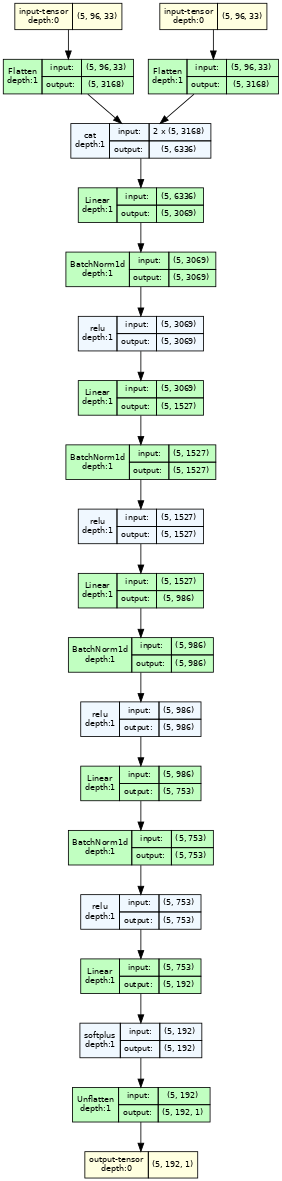
\includegraphics[width=0.5\textwidth]{chapters/3_models/imgs/ufcnmodel.png}
		\caption{Beseline Model architecture visualization.}\label{fig:baselinemodelarch}
	\end{minipage}
\end{figure}

\begin{minipage}[t]{0.5\textwidth}
	\begin{figure}[H]
		\centering
		\begin{tikzpicture}
			\draw[->] (-3,0) -- (3,0) node[right] {$x$};
			\draw[->] (0,-1) -- (0,4) node[above] {$y$};
			\draw[dotted] (-3,-1) grid (3,4);
			\draw[color=blue, domain=-3:0] plot[id=logistic] function{0};
			\draw[color=blue, domain=0:3] plot[id=logistic] function{x};
		\end{tikzpicture}
		\caption{Rectified Linear Unit function. $ReLu(x) = \max(0, x)$}
		\label{fig:relu}
	\end{figure}
\end{minipage}%
\hspace{.5cm}
\begin{minipage}[t]{0.5\textwidth}
	\begin{figure}[H]
		\centering
		\begin{tikzpicture}
			\draw[->] (-3,0) -- (3,0) node[right] {$x$};
			\draw[->] (0,-1) -- (0,4) node[above] {$y$};
			\draw[dotted] (-3,-1) grid (3,4);
			\draw[color=blue, domain=-3:3] plot[id=logistic] function{log(1+exp(x))};
		\end{tikzpicture}
		\caption{SoftPlus function. $SoftPlus(x) = \frac{1}{\beta} \log(1+e^{\beta x})$}
		\label{fig:softplus}
	\end{figure}

\end{minipage}

\subsection{Training}
\subsection{Evaluation}